\section{Download and Installation}
\label{sec:download-and-installation}
To install the softwares that are needed for the tasks, I firstly download the
installation script from the ftp server through wget command, give it the right
permissions to run and then run it.

\begin{figure}[H]
  \centering
  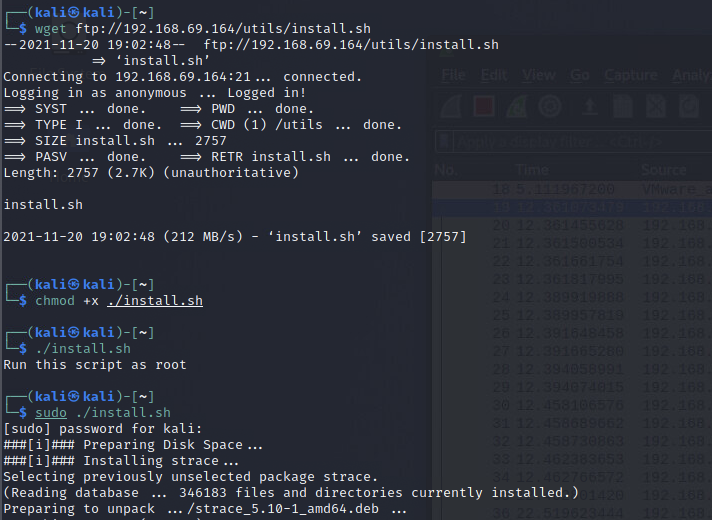
\includegraphics[width=0.6\textwidth]{figures/install-sh}
  \caption{Installation script}
  \label{f:install-sh}
\end{figure}

The application to reverse engineer is then downloaded as well.

\begin{figure}[H]
  \centering
  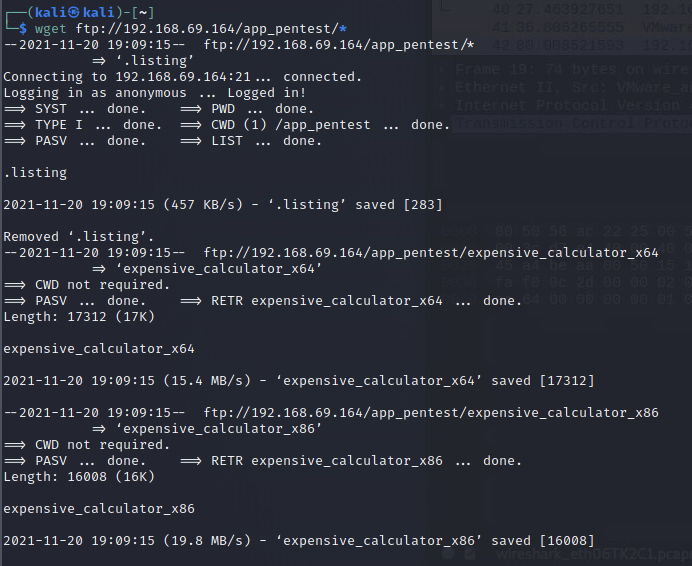
\includegraphics[width=0.6\textwidth]{figures/app_pentest}
  \caption{Folder apppentest}
  \label{f:app_pentest}
\end{figure}

The folder contains two files ending x64 and x86 and for this task I will be
working on the x84.

The output of the script is the following:

\begin{figure}[H]
  \centering
  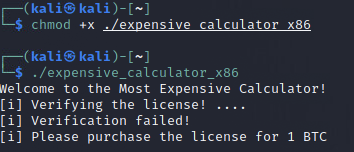
\includegraphics[width=0.6\textwidth]{figures/expensive_calculator_run}
  \caption{Expensive Calculator x86}
  \label{f:expensive_calculator_run}
\end{figure}

\section{Investigation}
\label{sec:investigation}


